% This chapter will introduce MHD modeling of Jupiter's magnetosphere.
% Need to explain the basic concept of MHD equations and perhaps a
% brief description of finite-volume methods, if necessary. It is
% important to cover 
%       - introductory text on the modeling of planetary magnetospheres
%       - the ionosphere solver and MI coupling in sufficient detail
%       - mass loading at Jupiter.
%       - This is a good place to discuss data model comparisons

\chapter{Model Description}

\blfootnote{*Parts of this chapter were published in - Sarkango, Y., Jia, X., \& Toth, G. (2019). Global MHD simulations of the response of Jupiter's magnetosphere and ionosphere to changes in the solar wind and IMF. Journal of Geophysical Research: Space Physics, 124.}

\section{Introduction}

Compared to the size of planetary magnetospheres, in situ coverage by spacecraft is sparse and only provides information about the immediate surroundings. In the past, when in-situ spacecraft were lesser in number, a global understanding of magnetospheric processes was limited to theoretical models, which used various assumptions to simplify the problem statement. After the development of faster computers, it became possible to simulate the magnetosphere by solving the magnetohydrodynamic equations in a large, three-dimensional domain using finite-difference or finite-volume methods \cite{Leboeuf1978GlobalMagnetosphere,Walker1989GlobalMagnetosphere,Ashour-Abdalla1985SpaceSimulations}. 

These global magnetospheric models were crucial to understanding the terrestrial magnetosphere from first-principles. However, they did not account for various phenomena which operate outside the fluid approximation, e.g. the ring current \cite{Fok1999ModelingSubstorms}, magnetic reconnection \cite{Birn2001GeospaceChallenge} etc. Since the early models, global models of the magnetosphere have been improved tremendously and increased in complexity. \citeA{Goodman1995ASimulations} proposed a technique to simulate the magnetosphere-ionosphere coupling by connecting the magnetospheric inner boundary with a Poisson solver for the electrostatic potential in the ionosphere. The Michigan Space Weather Modeling Framework (SWMF) coupled the magnetospheric finite-volume solver to dedicated models of the ring current \cite{DeZeeuw2004CouplingResults}. Improvements were made to simulate and understand the interactions between different particle species, instead of relying on a single-fluid \cite{Glocer2009MultifluidResults,Wiltberger2010InfluenceMagnetosphere}. \citeA{Meng2012PressureModel} extended the Michigan model by allowing for different plasma pressures along the directions parallel and perpendicular to the field lines. 

More recently, there has been increased interest to include kinetic-scale physics within the fluid magnetohydrodynamic models. Existing MHD models, although computationally efficient, cannot accurately predict the effect of magnetic reconnection on the plasma and the magnetosphere. On the other hand, particle-in-cell (PIC) models (e.g. \citeNP{Markidis2011TheMethod} and references therein), which are computationally expensive, have been found to simulate the kinetic processes well. The PIC method involves tracking the influence of the electromagnetic field (due to external or internal sources) on a collection of `particles', whose motion is modified due to the Lorentz force. Recent models have sought to combine the two approaches by embedding a smaller PIC region within a larger domain, where kinetic physics is considered to be important \cite{Daldorff2014Two-wayModel}. An alternative approach is to use higher-order moments of the Vlasov equation \cite{Wang2015ComparisonReconnection}, which also accounts for the missing physics in ideal MHD; the latter being derived using 3-moments .

Many attempts have been made to model Jupiter's magnetosphere, also trending towards an increasing degree of complexity. The first attempt was by \citeA{Miyoshi1997}, followed by the MHD model of \citeA{Ogino1998a}, which was used in multiple studies to model the Jovian bow shock and magnetopause \cite{Joy2002a} and to study magnetospheric currents and the solar wind‐magnetosphere interaction. \citeA{Walker2001} and \citeA{Fukazawa2006a} improved upon the model of \citeA{Ogino1998a} and investigated the dynamics of the magnetosphere such as the location, frequency of occurrence and characteristics of tail reconnection and plasmoid formation \cite{Fukazawa2010a}. \citeA{Moriguchi2008} studied magnetospheric currents using their global MHD model. \citeA{Chane2013a} developed an MHD model and used it to study the influence of mass loading due to Io on the magnetosphere. In subsequent studies \cite{Chane2017a,Chane2018}, they investigated the response of the magnetosphere to changes in the solar wind (specifically increases in solar wind dynamic pressure) and its influence on field‐aligned currents in the ionosphere. Recently, \citeA{Wang2018ModelingSimulation} and \citeA{Zhang2018AsymmetricSystems} have also developed an MHD model for Jupiter's magnetosphere.

Owing to its large size and fast wave-speeds in the inner regions, modeling Jupiter's magnetosphere is computationally challenging. Due to this reason, previous models had placed their inner boundary well beyond the orbit of Io, where mass loading is expected to occur. To account for the mass loading contribution, they had either employed a fixed boundary condition at the inner boundary, or changed the location of the Io torus altogether. For the same reason, all models of the Jupiter system, including the one discussed in this Chapter, solve the ideal MHD equations (with or without relativistic terms) without the aforementioned techniques used for the terrestrial system. One exception is the recent model by \citeA{Zhang2018AsymmetricSystems}, which uses two ion species - H$^+$ and O$^+$ to represent the population from the solar wind and from Io, respectively and is the first multi-fluid model of the Jovian system. 

In this chapter we introduce a new MHD model for Jupiter's magnetosphere based on the BATSRUS MHD code \cite{Powell1999a,Gombosi2002b}, which is coupled to the Ridley ionosphere electrodynamics solver \cite{Ridley2004IonosphericConductance}. Unlike previous MHD models, our model includes mass loading due to Io in a self‐consistent manner at the right location.

\subsection{The BATSRUS MHD model}
We use the Block-Adaptive Roe-type Solar wind Tree Upwind Scheme (BATSRUS) magnetohydrodynamic (MHD) solver to model Jupiter's magnetosphere in a self-consistent manner. BATSRUS uses a finite-volume approach and can be used as a component in the larger Space Weather Modeling Framework (SWMF) \cite{Toth2012a}, developed at the University of Michigan, which is a collection of models used in conjunction to simulate various space plasma phenomena. 

Over the years, BATSRUS has developed into an industry standard for simulating the space environment, especially in global magnetohydrodynamic modeling of planetary magnetospheres and has been used to simulate the magnetospheres of Earth, Mercury, Saturn \cite{Jia2012} and Jupiter \cite{Hansen2001a}, and also those of exoplanets. In this work, we use BATSRUS to solve the single-fluid, ideal, semi-relativistic MHD equations, repeated below from \citeA{Gombosi2002b} in the conservative form. 

\begin{equation}
    \frac{\partial \mathbf{W}}{\partial t} + \left(\nabla \cdot \mathbf{F} \right)^T = \mathbf{S}
\end{equation}

\begin{equation}
    \mathbf{W} = \left[ \begin{array}{c}
    \rho\\
    \rho \mathbf{u} + \frac{1}{c^2}\mathbf{S}_A\\ 
    \mathbf{B}     \\
    \frac{1}{2}\rho u^2 + \frac{p}{\gamma - 1} + e_A\\
    \end{array} \right]
\end{equation}


\begin{equation}
    \mathbf{F} = \left[ \begin{array}{c}
    \rho \mathbf{u}\\
    \rho \mathbf{u} \mathbf{u} + p\mathbf{I} + \mathbf{P}_A\\ 
    \mathbf{u}\mathbf{B} - \mathbf{B}\mathbf{u}\\
    \left(\frac{1}{2}\rho u^2 + \frac{\gamma p}{\gamma - 1}\right)\mathbf{u} + \mathbf{S}_A\\
    \end{array} \right]^T
\end{equation}

Where $\mathbf{W}$ is the state vector and $\mathbf{F}$ is the flux diad, comprising of the primitive variables - mass density $\rho$, plasma velocity $\mathbf{u}$, magnetic field intensity $\mathbf{B}$ and thermal pressure $p$. Note that in ideal MHD, the electric field is defined to be $\mathbf{E} = -\mathbf{u} \times \mathbf{B}$ (also called the motional electric field). The source terms ($\mathbf{S}$) on the right hand side will be discussed in a later section. $\mathbf{S}_A$, $e_A$, and $\mathbf{P}_A$ are the Poynting vector, electromagnetic energy density and electromagnetic pressure tensor.
\begin{align}
    \mathbf{S}_A & = \frac{1}{\mu_0} \mathbf{E} \times \mathbf{B}\\
    e_A &= \frac{1}{2\mu_0} \left( B^2 + \frac{1}{c^2} E^2\right)\\
    \mathbf{P}_A &= e_A \mathbf{I} - \frac{\mathbf{B}\mathbf{B}}{\mu_0} - \frac{1}{\mu_0 c^2}\mathbf{E}\mathbf{E}
\end{align}

The semi-relativistic equations are derived from the full relativistic MHD equations \cite{Gombosi2002b} by keeping the relativistic treatment of the electromagnetic terms while assuming that the plasma flow itself is non-relativistic. The use of semi-relativistic or fully relativistic MHD equations is crucial to accurately simulate Jupiter's magnetosphere since the Alfven speeds near the polar regions of the planet approach the speed of light due to the strong planetary magnetic field. This is a major limitation on numerical models, as the Courant–Friedrichs–Lewy criteria specifies that the simulation time step in time-accurate simulations using explicit time-stepping be lower than that determined roughly by the ratio of the grid spacing and the maximum wave speed in the system. Typically, the maximum wave-speed in the system is further limited to a fraction of the speed of light, also called the Boris correction \cite{Toth2011}. In our simulations the Boris correction factor is chosen to be either 0.1 or 1 (no Boris correction), depending on the problem. A detailed description of the implementation for BATSRUS can be found in the literature \cite{Gombosi2002b, Toth2012a}.

Our MHD model for Jupiter's magnetosphere utilizes the Space Weather Modeling Framework (SWMF) developed at the University of Michigan \cite{Toth2012a} and is an extension of the model used by \cite{Hansen2001a}. Two modules of the SWMF are used — a magnetospheric solver that employs BATSRUS \cite{Gombosi2002b,Powell1999a}, and a Poisson solver for the ionospheric electrodynamics \cite{Ridley2004IonosphericConductance}, and the two modules are two‐way coupled through the SWMF.  The planetary magnetic field currently used in our model is a dipole with an equatorial surface field strength of 428000 nT, and the rotation period of the planet is set to be 10 hours. While we initially set the magnetic axis to the aligned with the rotation axis, in Chapter 5 we also present the results from simulations using a non-axisymmetric internal field, which represents more realistically the situation as observed at Jupiter. 

\begin{figure}
    \centering
    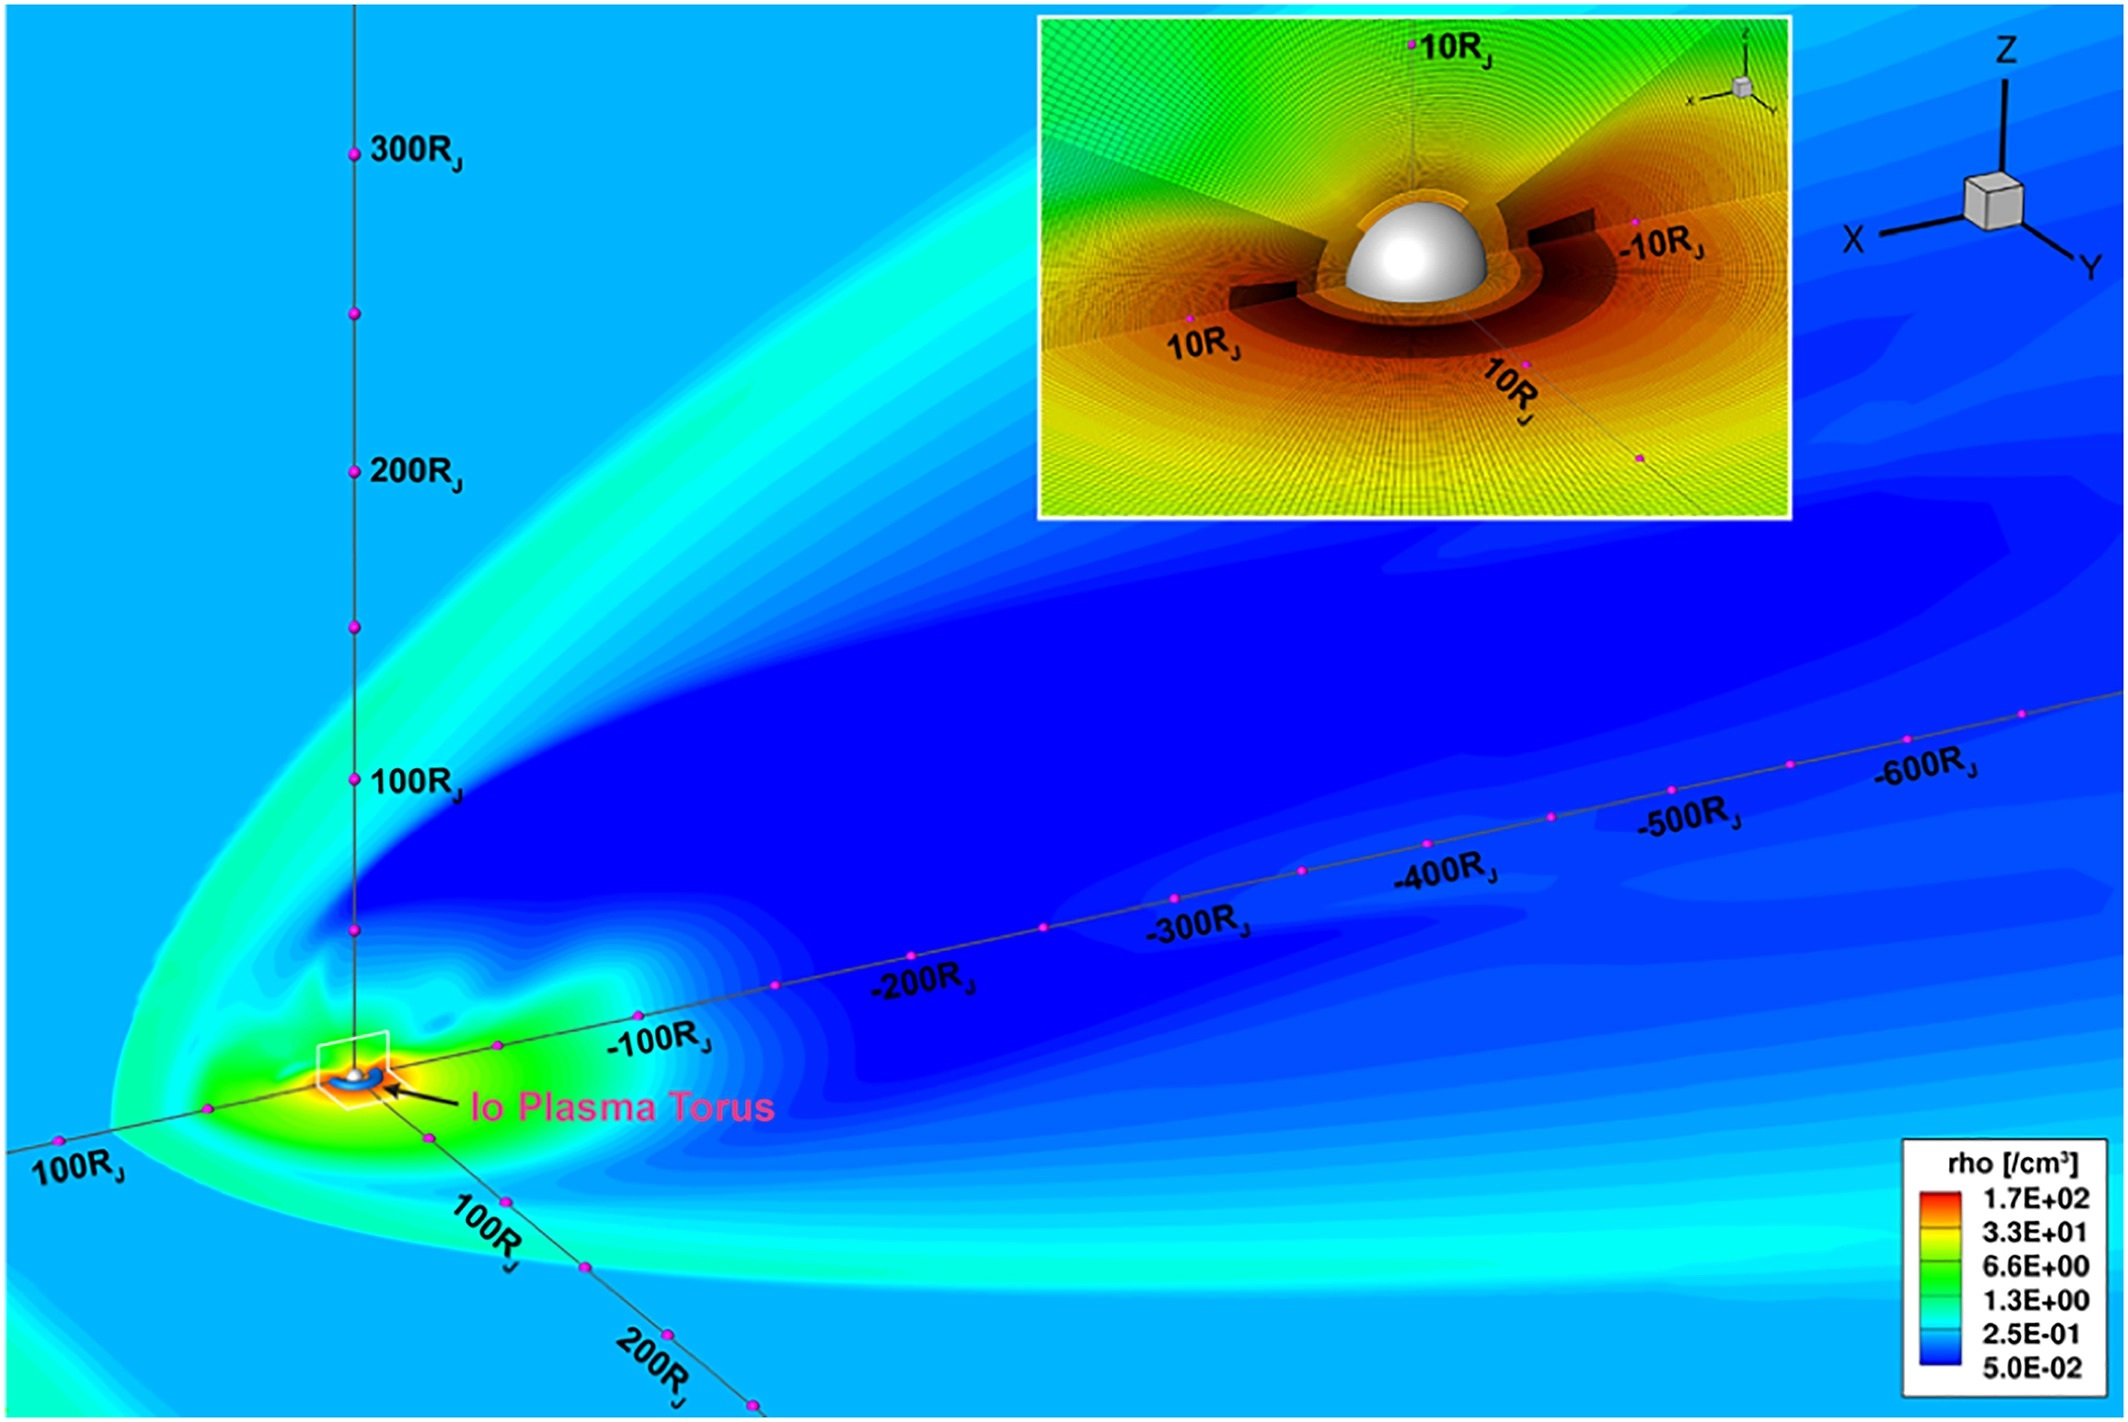
\includegraphics[width=0.8\textwidth]{images2/global-mhd-image.jpg}
    \caption{A global view of Jupiter's magnetosphere as modeled by BATSRUS. Plasma density contours are shown in the $z=0$ and $y=0$ plane. The inset shows the regions close to the planet, where various grid refinements can be seen. The Io torus is located at a radial distance of 6 $R_J$ from the planet.}
    \label{fig:global-mhd-image}
\end{figure}

Our three‐dimensional magnetospheric simulation domain spans a spherical region of 1800 $R_J$ centered at Jupiter, along with a planar cut at $X$ = 192 $R_J$ that serves as the upstream boundary (Figure \ref{fig:global-mhd-image}). The radial spacing between the grid cells increases in a logarithmic manner allowing for finer cells placed in regions close to the planet. The simulation domain is subdivided into a number of blocks \cite{Powell1999a}, which can be refined independently to obtain the desired grid resolution in regions of interest, such as the equatorial magnetosphere, the magnetopause boundary, and the magnetotail. Although BATSRUS allows for physics criteria‐based adaptive grid refinements \cite{Toth2012a}, in our simulations the refinements are prescribed initially and are fixed. The spherical inner boundary of our simulation domain is located at 2.5 $R_J$, which then allows us to include the Io plasma torus centered at $\sim$5.9 $R_J$, which is the appropriate location. We specifically chose to refine a torus‐like region near Io's orbit for accurately modeling the mass loading processes occurring in the Io plasma torus. The smallest radial grid spacing is $\sim$0.06 $R_J$, which is present in the Io plasma torus. Figure \ref{fig:global-mhd-image} shows our simulation grid with contours of simulated plasma density shown in the background for context. The relatively coarse grids near the polar regions of the planet were chosen to allow for larger time steps in order to increase the speed of the simulation, as these regions contain strong magnetic fields and thus high wave speeds as well as small grid cells due to the convergence of the spherical grid near the $Z$ axis. 

All MHD variables at the upstream boundary at $X$ = 192 $R_J$ are prescribed on account of the super‐Alfvenic and supersonic solar wind flow, whereas floating boundary conditions that set zero gradients for all MHD variations are applied at the outer boundary in the downstream direction (located at -1800 $R_J$). At the inner boundary at 2.5 $R_J$, we fixed the plasma density at 50 amu/cm$^3$ and set the magnetic field and plasma pressure to \emph{float} i.e. take on values similar to the nearest MHD cell. Using the electrostatic potential calculated by the ionosphere electrodynamics Poisson solver (discussed later), we calculate the electric field ($\mathbf{E}$) at the inner boundary. The $\mathbf{E} \times \mathbf{B}$ velocity thus obtained is added to the corotation velocity ($\mathbf{u_c} = -\mathbf{\omega} \times \mathbf{r}$) at the inner boundary.

The fluxes at cell interfaces used in the finite‐volume method are calculated using a second‐order accurate implementation of Linde's HLL scheme \cite{Linde2002}. To achieve computational speeds feasible for running long‐duration simulations, we employ a hybrid time‐stepping scheme. Explicit time‐stepping methods are subject to the Courant‐Friedrichs‐Lewy criterion that imposes a stringent constraint on the allowable time step, which may become rather small in regions of high wave speeds, such as the polar region near the planet. Implicit time‐stepping schemes are unconditionally stable and therefore allow larger time steps but involve matrix inversion, which can be computationally expensive for large systems. To combine the strengths of these two methods, we use an “explicit/implicit” hybrid time‐stepping algorithm developed by \cite{Toth2006AGrids}. Since our domain is divided into grid blocks, with each block containing $6 \times 8 \times 8$ cells, this algorithm allows for each block to be solved using either explicit or implicit time stepping for a prescribed value of the computational time step. Blocks in which all cells abide by the CFL criterion defined for the time step are solved using explicit time stepping. In total, our finite‐volume grid contains approximately 19 million cells, and with a 20‐s time step our global model can achieve almost real‐time performance using $\sim$2000 cores on NASA's supercomputer Pleiades or the Frontera supercomputer at the University of Texas.

\subsection{The Ridley Ionosphere Electrodynamics solver}
The IE solver operates under an electrostatic assumption and solves for the electrostatic potential on a spherical surface of radius $R_1=1$ R$_J$ using the Poisson equation \cite{Ridley2004IonosphericConductance}.
\begin{equation}
    j_R \left(R_1\right) = \left[ \nabla_\perp \cdot \left( \mathbf{\Sigma} \cdot \nabla \psi \right) \right]_{r=R_1}
\end{equation}

Where $j_R$ is the current density in the radial direction, $\psi$ is the electrostatic potential on the surface and $\mathbf{\Sigma}$ is the height-integrated conductance tensor which, in a local cartesian coordinate system where $Z$ in the direction of the magnetic field, takes the form 
\begin{equation}
    \mathbf{\Sigma}' = \left[ \begin{array}{ccc}
    \Sigma_P     &-\Sigma_H   &0  \\
    \Sigma_H     &\Sigma_P   &0  \\
    0          &0        &\Sigma_0
    \end{array} \right]
\end{equation}

With $\Sigma_H$, $\Sigma_P$ and $\Sigma_0$ being the Hall, Pedersen and Alfven conductance respectively. The conductance is derived from the respective conductivity by integrating along the radial (height) direction \cite{Goodman1995ASimulations}. 

\begin{equation}
\Sigma_i = \int_{r_1}^{r_2} \sigma_i \, dr
\end{equation}

The IE solver uses a finite-differencing method to construct the linear system which is solved using iterative methods separately for the northern and southern hemispheres.

Two‐way coupling between BATSRUS and the IE solver is achieved in the following manner. Field‐aligned currents from the magnetosphere are collected at a prescribed radial distance of 3 $R_J$ ($R_J$ = 71492 km is Jupiter's mean radius at 1 bar pressure) and are then mapped to the surface of the planet assuming that the magnetic field between 1 and 3 $R_J$ is dipolar. At the surface, a Poisson solver is used to solve Ohm's law for a given distribution of ionospheric conductance. In the present work, we assume a uniform Pedersen conductance of either 0.05 S or 0.1 S, which is on the lower end of previous estimates (0.1–10 S by \citeNP{Strobel1983Ionosphere,Nichols2003} and 0.47 S by \citeNP{Gerard2021VariabilityAurora}) and set the Hall conductance to 0. The perturbation electric field obtained from the IE module is added to the co-rotational electric field, and the total electric field is then used to prescribe the plasma velocity at the inner boundary of the MHD domain at 2.5 $R_J$. A detailed discussion of how this coupling is achieved is given by \citeA{Ridley2004IonosphericConductance} in the context of the terrestrial magnetosphere and by \citeA{Jia2012} and \citeA{Jia2012DrivingSources} in application to Saturn's magnetosphere.

\subsection{Mass loading sources terms}
In order to accurately model Jupiter's magnetosphere, it is necessary to include the contribution of plasma by its moons, especially Io. Io provides the largest internal source of plasma to Jupiter's magnetosphere, estimated to add $\sim$250 kg/s to 1 ton/s of plasma \cite{Bagenal2011b}. In our model, we include contributions due to ionization and charge‐exchange in the form of source terms in the mass, momentum, and energy equations. Dissociative recombination is a minor process and, therefore, neglected in the present simulations. We use a prescribed neutral torus centered at Io's orbital radius of 5.9 $R_J$ according to the following form. The neutral distribution used for the Io torus is a modified form of the one obtained by \citeA{Schreier1998a} and an exponential falloff with latitude is considered. We prescribe the following expression to calculate the neutral number density ($n_n$ [cm$^{-3}$]) at a spatial location defined in terms of cylindrical coordinates ($r_{xy} = \sqrt{x^2 + y^2}$ $R_J$). 

\begin{equation}
    n_n \left(r_{xy}, z\right) = n_{n_0} \exp{\left(\frac{-z^2}{H_s^2}\right)}\times 
    \begin{cases}
        60 \exp\left( \frac{r_{xy} - 5.71}{0.2067}\right), & r_{xy} < 5.71\\
        60 \exp\left( \frac{-r_{xy} + 5.685}{0.1912}\right), &
        5.71 \leq r_{xy} < 5.875\\
        19.9 \exp\left( \frac{-r_{xy} + 5.9455}{0.0531 r_{xy} + 0.5586 }\right), &r_{xy} >= 5.875
    \end{cases}
\end{equation}

Where the scale height is chosen to be $H_s = r_{xy} \tan^{-1}2.5^\circ$. New ions are produced from the above neutral distribution by multiplying with a constant ionization rate and collision cross section based on the following expression for the net plasma production rate per unit volume (units of kg m$^{-3}$ s$^{-1}$):

\begin{equation}
    \dot{\rho} = 16 m_p n_n C_i
\end{equation}

Here $C_i$ is the ionization rate (specified to 10$^{-4}$ s$^{-1}$ in our simulations) and 16 amu is taken to be the average mass of the heavy ions present in Jupiter's magnetosphere. Figure \ref{fig:mass-loading} shows the contours of the ionization source ($\dot{\rho}$) in the plane perpendicular to the equator. With this information, we construct the source term $\mathbf{S}$ for the mass continuity, momentum, total energy and thermal energy equations \cite{Hansen2001a, Gombosi1996Three-dimensionalEnvironments}: 

\begin{figure}
    \centering
    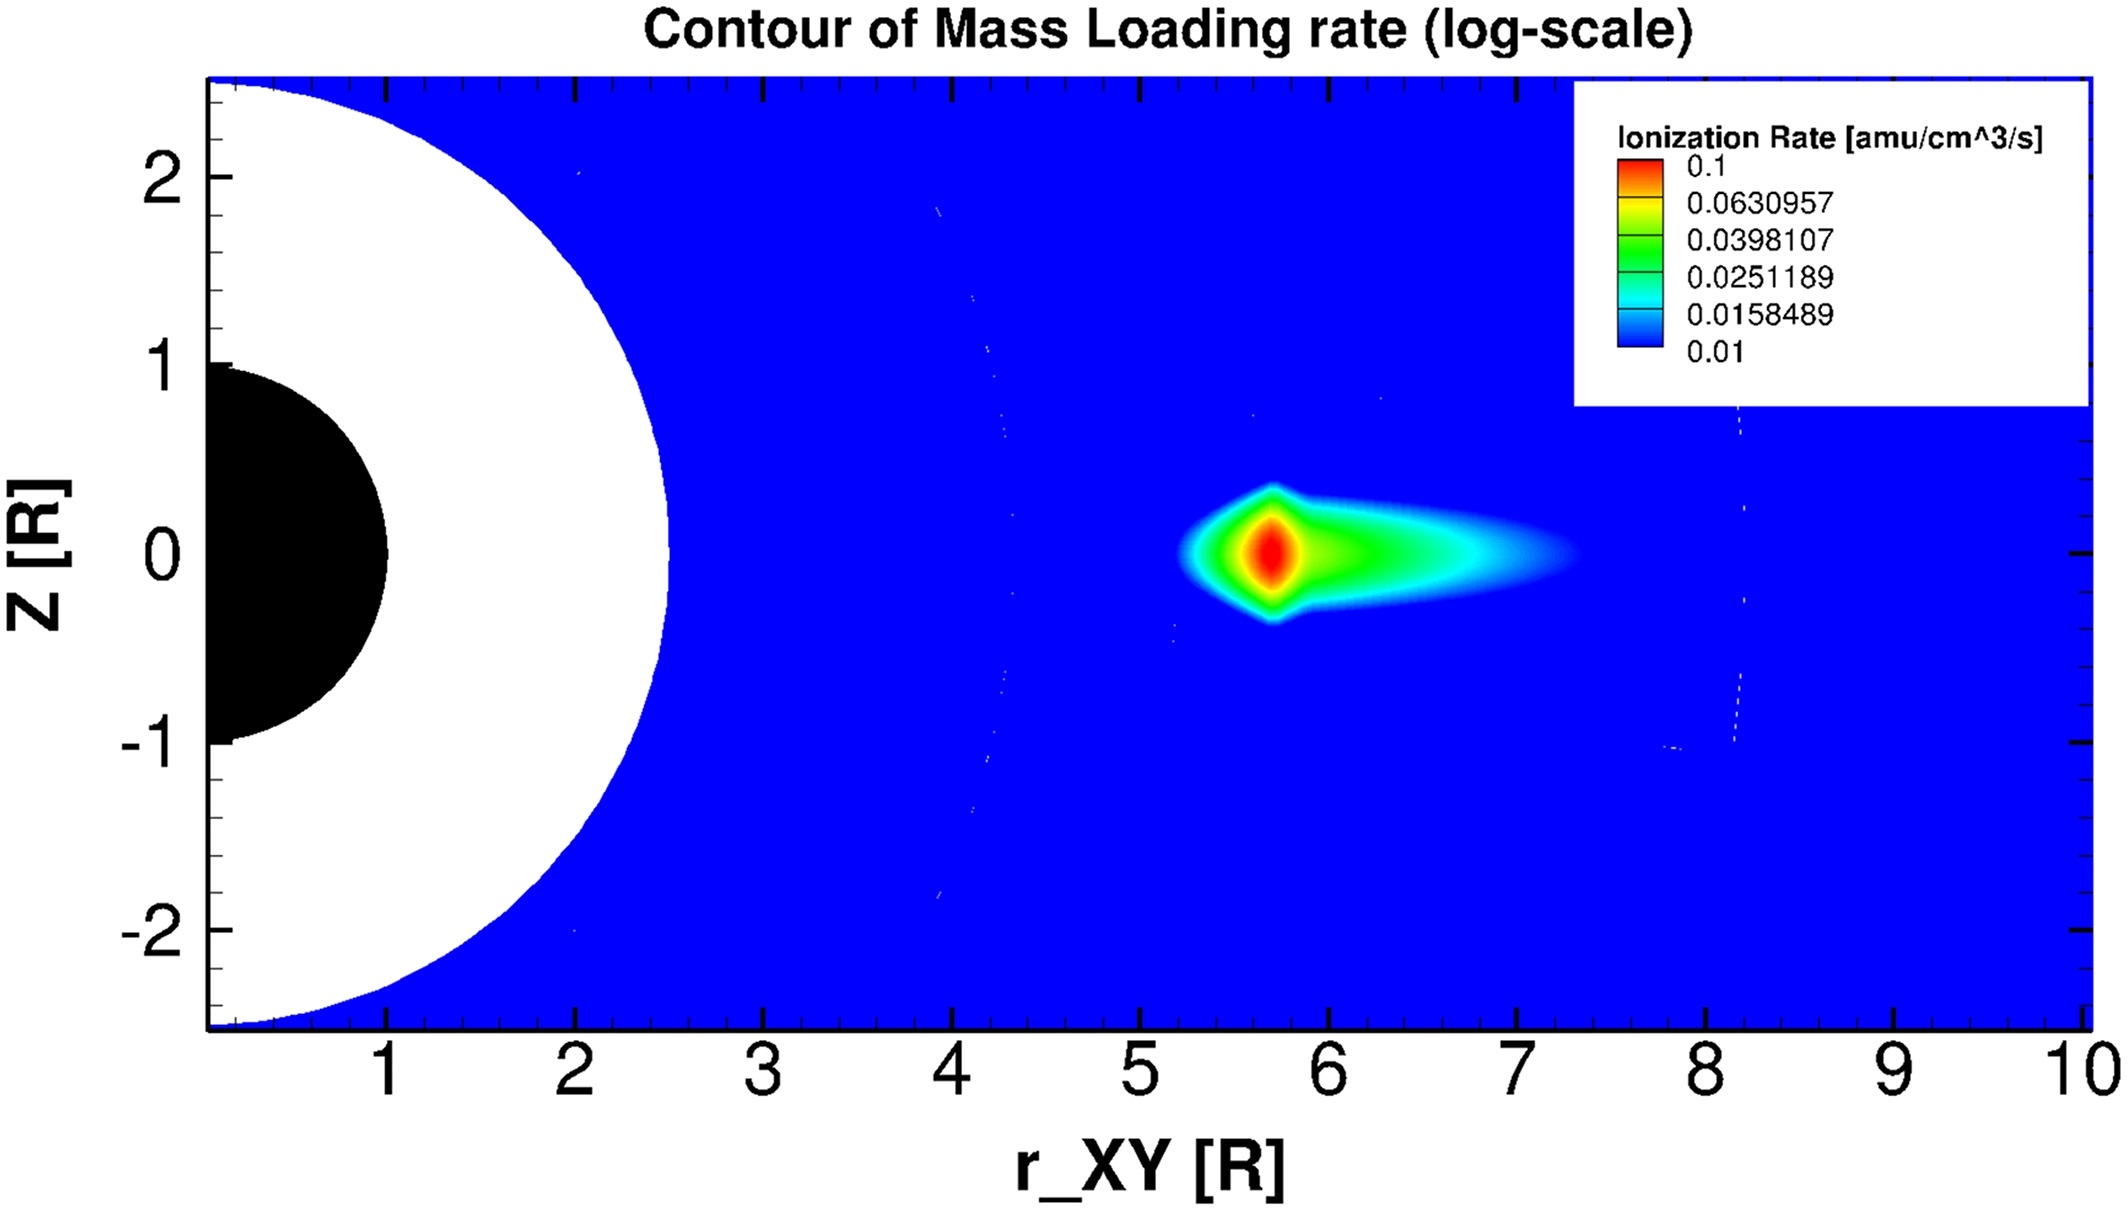
\includegraphics[width=0.8\textwidth]{images2/mass-loading.jpg}
    \caption{Contours of the mass loading source $\dot{\rho}$ in the meridional plane. The inner boundary is at 2.5 $R_J$ and the gap region between the magnetosphere and ionosphere is shown in white.}
    \label{fig:mass-loading}
\end{figure}

\begin{align}
    S_\rho & = \dot{\rho} - \alpha \rho \\
    S_{\rho U_x} & = \left(\dot{\rho} - C_x\right) u_{nx} - \left( C_x + \alpha \right) \rho u_x \\
    S_{\rho U_y} & = \left(\dot{\rho} - C_x\right) u_{ny} - \left( C_x + \alpha \right) \rho u_y \\
    S_{\rho U_z} & = -\left( C_x + \alpha \right) \rho u_z \\
    S_E & = \frac{1}{2} \left( \dot{\rho} + C_x \rho \right) u_n^2 - \frac{1}{2} \rho u^2 \left( C_x - \alpha \right) - \frac{3}{2} \alpha p + \frac{3}{2} C_x p \\
    S_p & = \frac{1}{2} \left( \dot{\rho} + C_x \rho \right) \left| \mathbf{u} - \mathbf{u}_n\right|^2 - \frac{3}{2} \alpha p 
\end{align}

Where $C_x = \dot{\rho} - n_n \sigma \left|\mathbf{u} - \mathbf{u}_n\right|$ is the charge exchange rate, $\mathbf{u}_n$ is the Keplerian velocity of the neutral particles orbiting Jupiter, and $\alpha$ is the recombination rate, which is set to 0 in our current work. As described above, the ion production rate in our simulation is a controlled parameter depending on the neutral profile, ionization rate, and collision cross section. In the present work, we set the total ion production rate of $\sim$1 ton/s. It is important to note that our approach of modeling the Io plasma torus is very different from those adopted by the previous Jupiter global MHD models. For instance, the \citeA{Miyoshi1997} MHD model had its inner boundary at 30 $R_J$. The inner boundary of the MHD model by \citeA{Ogino1998a} and \citeA{Fukazawa2005,Fukazawa2006a,Fukazawa2010a} lied at 15 $R_J$, while the \citeA{Moriguchi2008} model had its inner boundary at 8 $R_J$. The recent MHD model by \citeA{Chane2013a,Chane2017a} used an extended ionospheric region spanning from 4.5 to 8.5 $R_J$ and placed the Io torus at an unrealistic location of 10 $R_J$. In their recent model, \citeA{Wang2018ModelingSimulation} also chose to place the Io torus at 10 $R_J$ for the same reasons. Our model is the first global MHD model which models mass loading due to Io in a self‐consistent manner at the right location.

The above mass loading parameters were chosen based on ad-hoc assumptions to provide an equivalent mass loading rate of 1 ton/s. In practice, other neutral profiles can also be used, but regions with high plasma density gradients, such as the Io plasma torus usually have higher rates of numerical diffusion, which can diffuse the initially prescribed density distribution. 

\section{Magnetospheric configuration}
To create the magnetosphere, we use steady solar wind conditions with a southward (negative $B_Z$ ) IMF (values are given in column 1 of Table 1) to minimize reconnection at the start of the simulation. We speed up the creation of the magnetosphere by using local time stepping \cite{Toth2012a} for 50000 iterations and then switch to time‐accurate mode for 150 hr to produce a quasi‐steady state magnetosphere. All simulations presented in this paper have been started either from this point or a later time step. Because of the large system size and long time scales involved in Jupiter's global magnetosphere, it is necessary to use the procedure described above in order to ensure that simulation results shown and discussed here are not from a period dominated by the initial transients.


\section{Comparisons with in-situ data}

\begin{figure}
    \centering
    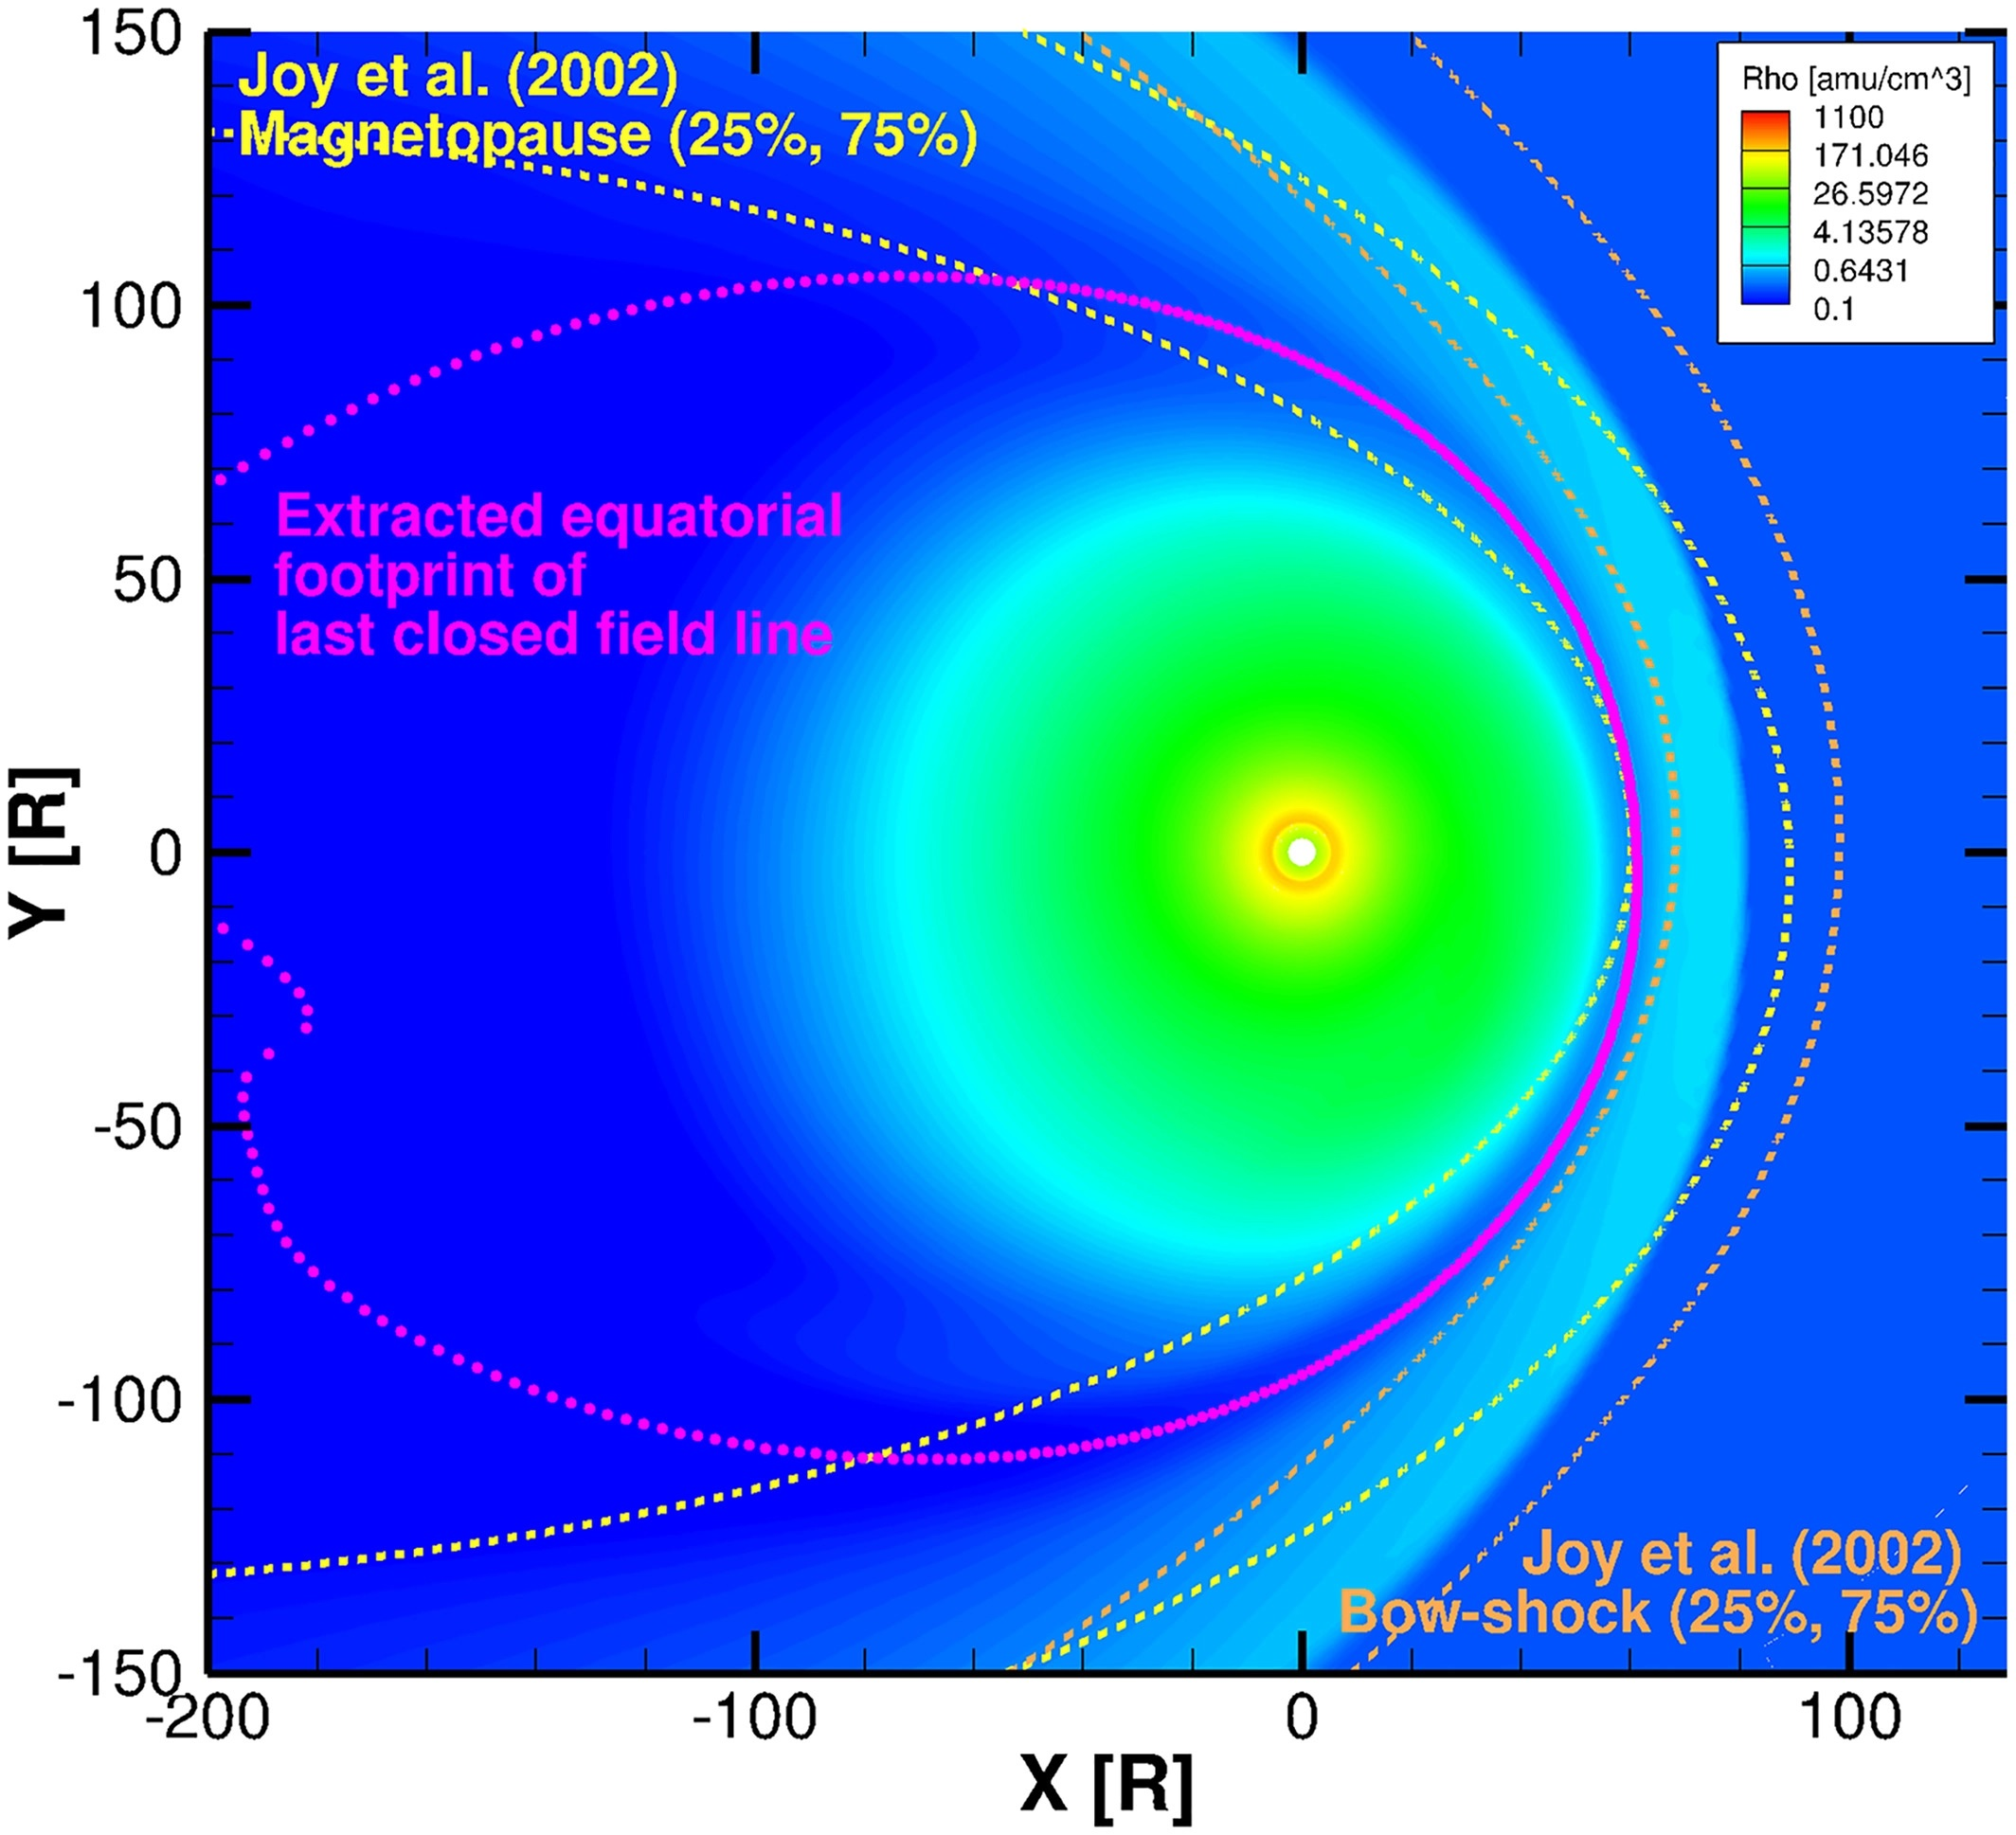
\includegraphics[width=0.7\textwidth]{images2/magnetopause-xy.jpg}
    \caption{Contours of plasma density in the equatorial plane in the MHD simulation. The dashed lines represent the magnetopause and bow-shock locations from the probabilistic model of Joy et al. (2002). The magenta points represent the location of the last closed field line, which corresponds to the magnetopause location on the dayside.}
    \label{fig:magnetopause-xy}
\end{figure}

To validate our global simulation model, we first present a set of comparisons of our MHD model results with available empirical models and in situ measurements. Figure \ref{fig:magnetopause-xy} shows a snapshot of the magnetospheric configuration in the equatorial ($XY$) plane extracted from the simulation using fixed nominal solar wind conditions and a southward IMF (Run 1 in Table 1) after it has reached quasi‐steady state. Results are presented in a Jupiter‐centered Cartesian coordinate system, where $X$ points toward the Sun, $Z$ is the magnetic and rotational axis (since dipole tilt is ignored in this simulation), and $Y$ completes the right‐handed coordinate system. The colors show contours of plasma density in logarithmic scale. The magenta points in the equatorial plane are the extracted equatorial footprints of the last closed field lines, which, on the dayside, correspond to the magnetopause in our model. The bow shock in our model can be readily identified as the separatrix between the unperturbed solar wind and the magnetosheath containing high‐density plasmas. Also plotted are the 25\% and 75\% probability curves from the \cite{Joy2002a} magnetopause and bow shock models assuming the same upstream solar wind pressure as used in our simulation. The comparison shows that the modeled magnetopause and bow shock fall well within the ranges predicted by the \citeA{Joy2002a} empirical model. It is, however, worth noting that while the modeled magnetospheric boundaries, in general, have a good agreement with observations, the size of the magnetosphere is slightly underestimated, due in part to absence of energetic particle pressure in our MHD model. 

\begin{figure}
    \centering
    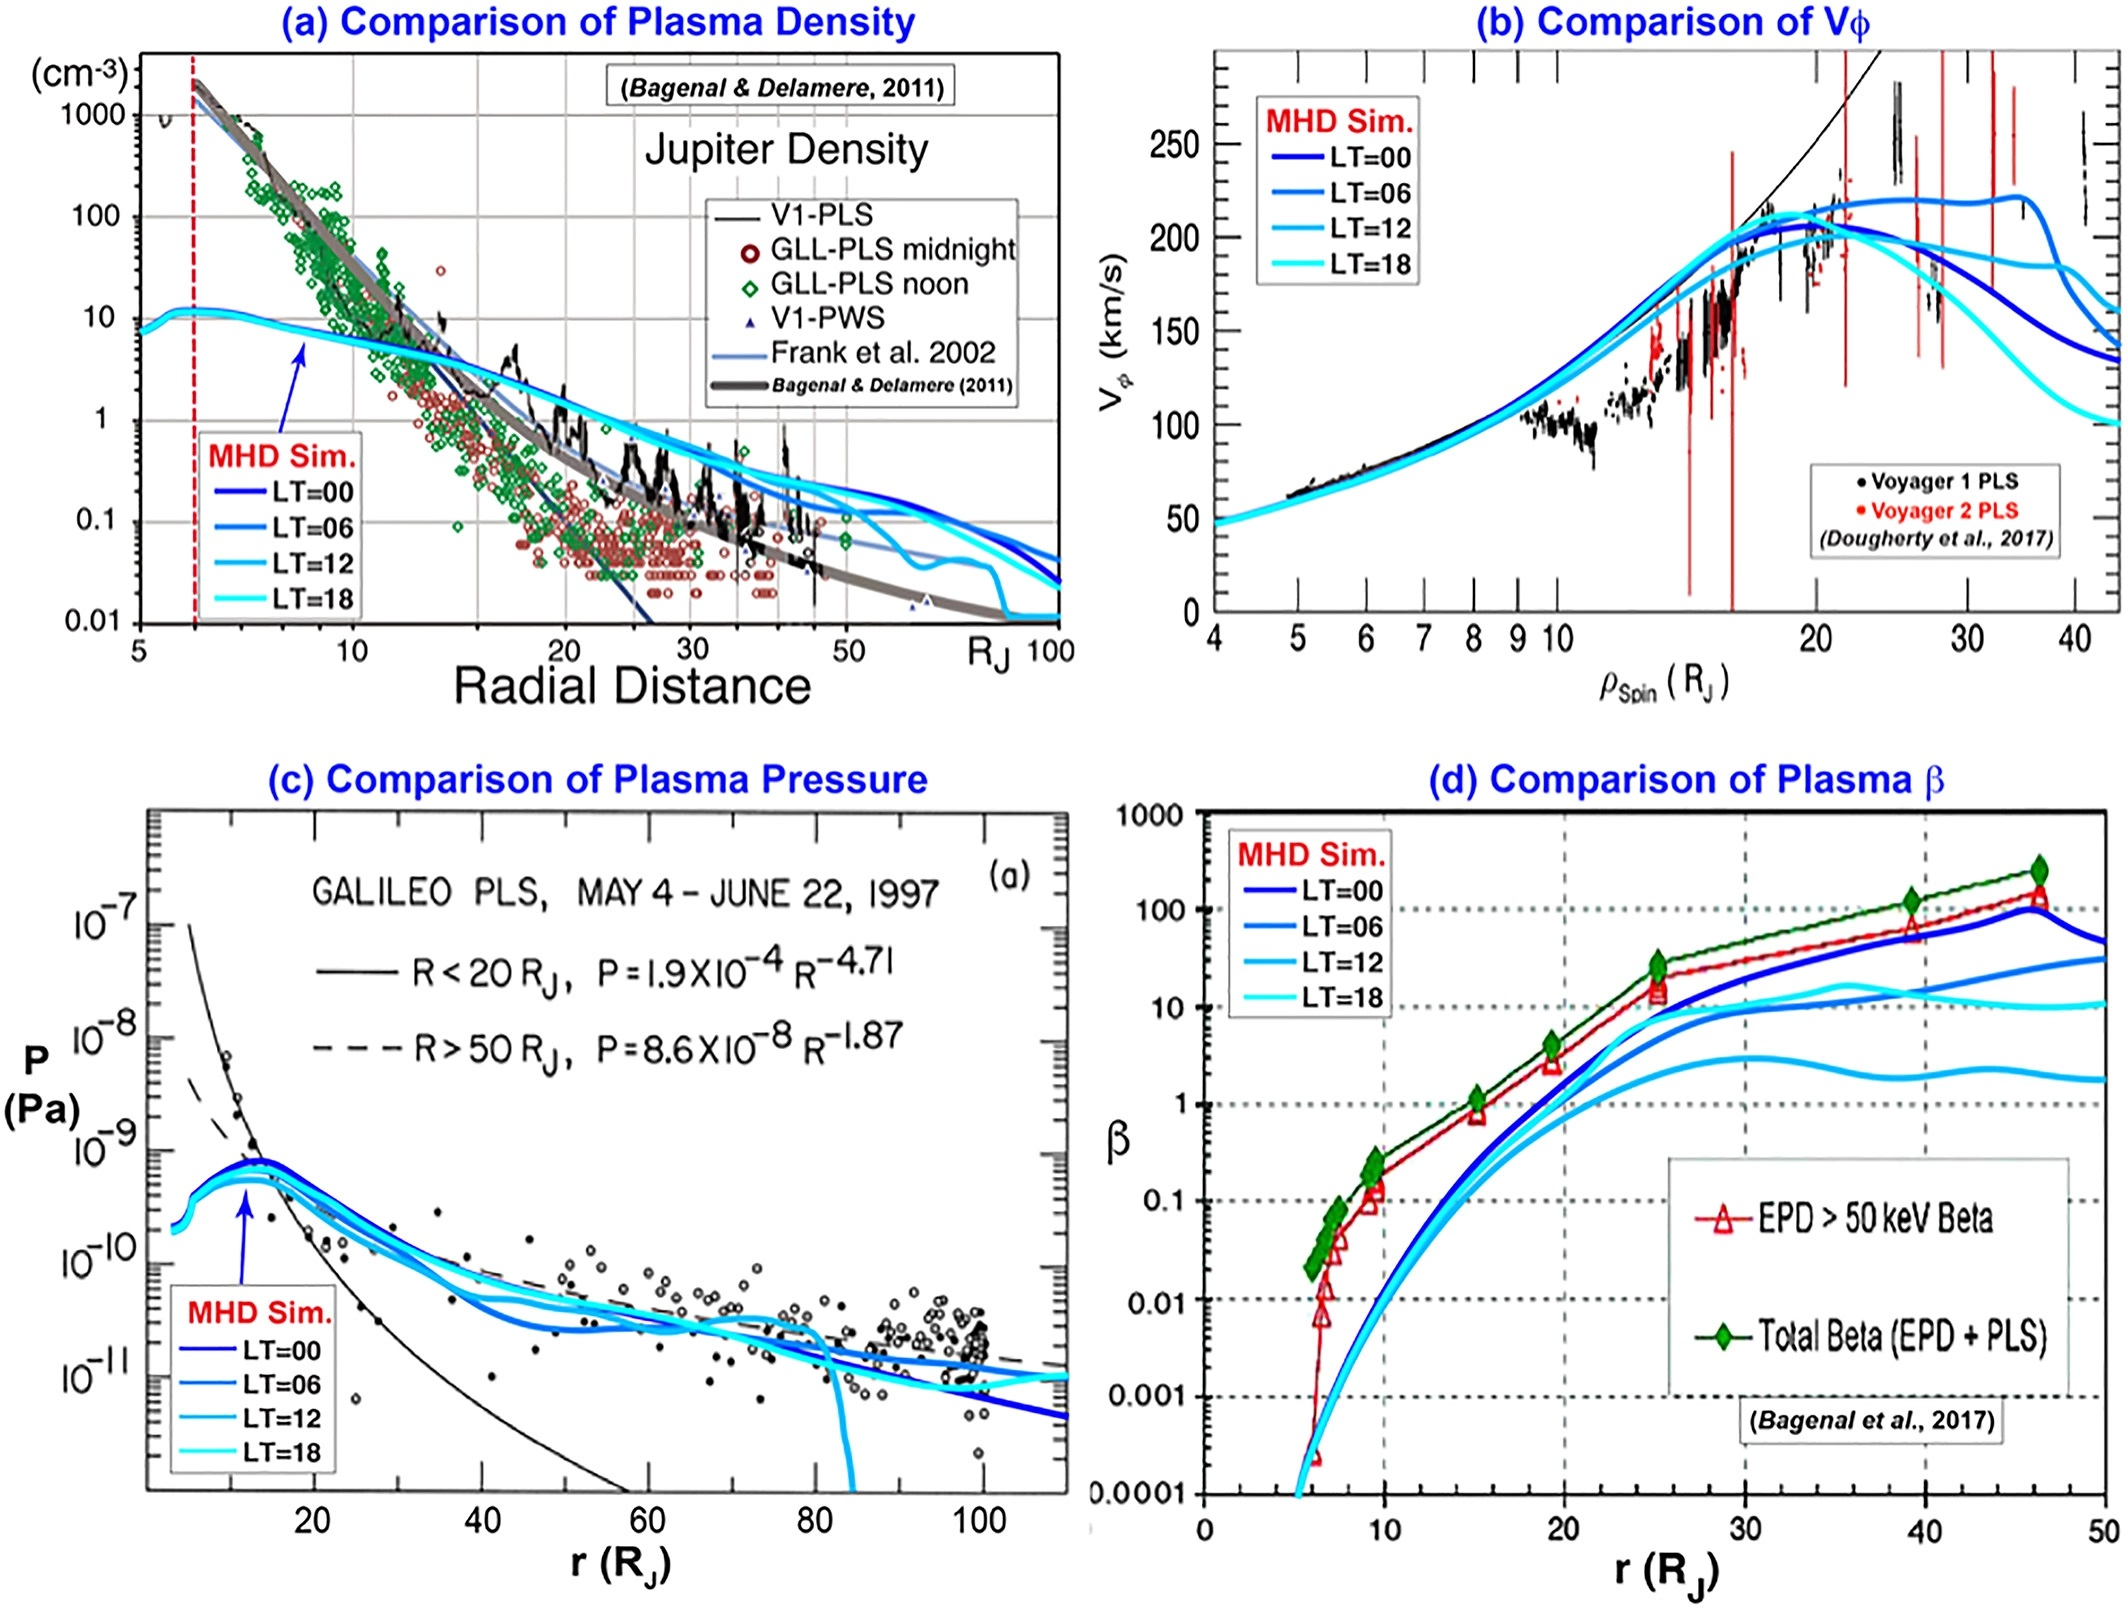
\includegraphics[width=\textwidth]{images2/comparison-plasma.jpg}
    \caption{Comparisons of the plasma parameters between our global MHD model and observations. In each panel, there are four traces extracted from the MHD model representing the radial profiles at four different local times (LT = 00, 06, 12, 18). (a) Plasma density. The compilation of density profiles based on Voyager and Galileo measurements is adapted from \protect\citeA{Bagenal2011b}. (b) Plasma azimuthal velocity ($V_\phi$). Voyager 1 and Voyager 2 PLS data are shown as black and red dots (with error bars; adapted from \protect\citeNP{Dougherty2017}). The black curve shows the rigid corotation speed for reference. (c) Plasma thermal pressure. The circles show the plasma pressures measured by Galileo PLS, while the black solid and dashed curves show fits to the data (adapted from \protect\citeNP{Frank2002}). (d) Plasma $\beta$. The red symbols and lines show the $\beta$ that only includes Galileo EPD‐measured energetic particle pressure contribution, whereas the green symbols and lines show the total $\beta$ when both EPD and PLS measured pressures are included (adapted from \protect\citeNP{Mauk2004}).}
    \label{fig:comparison-plasma}
\end{figure}

As another step in our model validation, we compare in Figure \ref{fig:comparison-plasma} the radial distribution of simulated plasma parameters with available in situ observations. In analyzing our simulation output, it became clear to us that the magnetosphere exhibits strong local time asymmetries and temporal variabilities. Therefore, in order to obtain a fair comparison with satellite data, which were collected in different local time sectors and in different magnetospheric states, we extracted simulation outputs in different local time meridians (LT = 0, 6, 12, and 18) and also from different time steps that cover both the southward (Run 1) and spiral IMF (Run 3) cases. Figure \ref{fig:comparison-plasma}a shows the time‐averaged radial profiles of the simulated plasma density in the central plasma sheet (blue/cyan curves), in comparison with a compilation of density profiles obtained from previous missions (adapted from \citeA{Bagenal2011b}). The density in the inner magnetosphere (inside $\sim$10 $R_J$) are significantly underestimated in our simulation, whereas it matches the observations in the middle and outer magnetosphere ($>$10 $R_J$) generally well. Several factors may contribute to the discrepancy seen in the inner magnetosphere. For instance, the grid resolution in the torus region, albeit relatively fine, may not be high enough to resolve the small scale height associated with the torus. Moreover, plasma pressure is assumed to be isotropic in our ideal MHD model, but anisotropies in plasma pressure may develop in regions where ion pickup occurs, for example, in the torus. Pressure anisotropies ($p_\perp > p_\parallel$) would cause the plasma to be more confined to the centrifugal equator (e.g., as discussed by \citeA{Dougherty2017}). However, because of the isotropic pressure assumption in our current ideal MHD model, the modeled plasma sheet in the inner magnetosphere is thicker than observed, which contributes to the underpredicted densities near the equator as shown in Figure \ref{fig:comparison-plasma}a. 

Figure \ref{fig:comparison-plasma}c shows a comparison of our modeled plasma pressure with the Galileo Plasma Science (PLS) measurements \cite{Frank2002}. Again, our model predicts lower pressures than observed in the inner magnetosphere, because of the lower densities discussed above. Nevertheless, the modeled pressure has a satisfactory agreement with the observations in the middle and outer magnetosphere ( $ >\sim15 R_J$). Figure \ref{fig:comparison-plasma}d compares our modeled plasma $\beta$ with Galileo observations \cite{Mauk2004}. The observations show that the plasma $\beta < 1$ in the inner magnetosphere and $\beta > 1$ in the middle/outer magnetosphere, and it crosses unity around 15 $R_J$. Our model results show a very similar general trend, although our modeled plasma $\beta$ tends to be lower than the observations due to the underestimation of density and absence of energetic particle pressure. However, in the middle and outer magnetosphere, our simulated $\beta$ appears to have a good agreement with the observations, especially in the nightside region. Our model also suggests that there is a considerable variability in the plasma $\beta$ among different local time sectors (largest near the midnight sector and smallest near noon sector), which is important to consider when it comes to model‐data comparison. 

Figure \ref{fig:comparison-plasma}b presents a validation of the plasma azimuthal velocity. The radial profile of the azimuthal velocity provides important constraints on models of plasma transport and magnetosphere‐ionosphere coupling, as demonstrated by a number of previous studies \cite{Cowley2001a,Hill1979,Hill1980,Nichols2011,Nichols2004,Pontius1997}. The observations show that the plasma flow starts to deviate significantly from rigid corotation around 20 $R_J$, where the corotation enforcement currents start to develop \cite{Cowley2001a,Hill2001}. In comparison, our modeled flow profiles show a very similar behavior in that the corotation breakdown occurs at about 15–20 $R_J$, in general agreement with the observations. The simulated azimuthal flows in all local time sectors are subcorotating outside of ~20 $R_J$, with a strong dependence on local time varying between 150 and 210 km/s at $\sim$30 $R_J$, which may account for the relatively large scattering of the measured flow velocities in this region. One feature in the observations that is not captured by our model is the deviation of the plasma flow from rigid corotation between 9 and 15 $R_J$. Plasma subcororation in this region so deep inside the magnetosphere was not predicted in the previous theoretical and numerical models. The physical cause of this behavior remains unidentified at present, and requires further investigation.

\begin{figure}
    \centering
    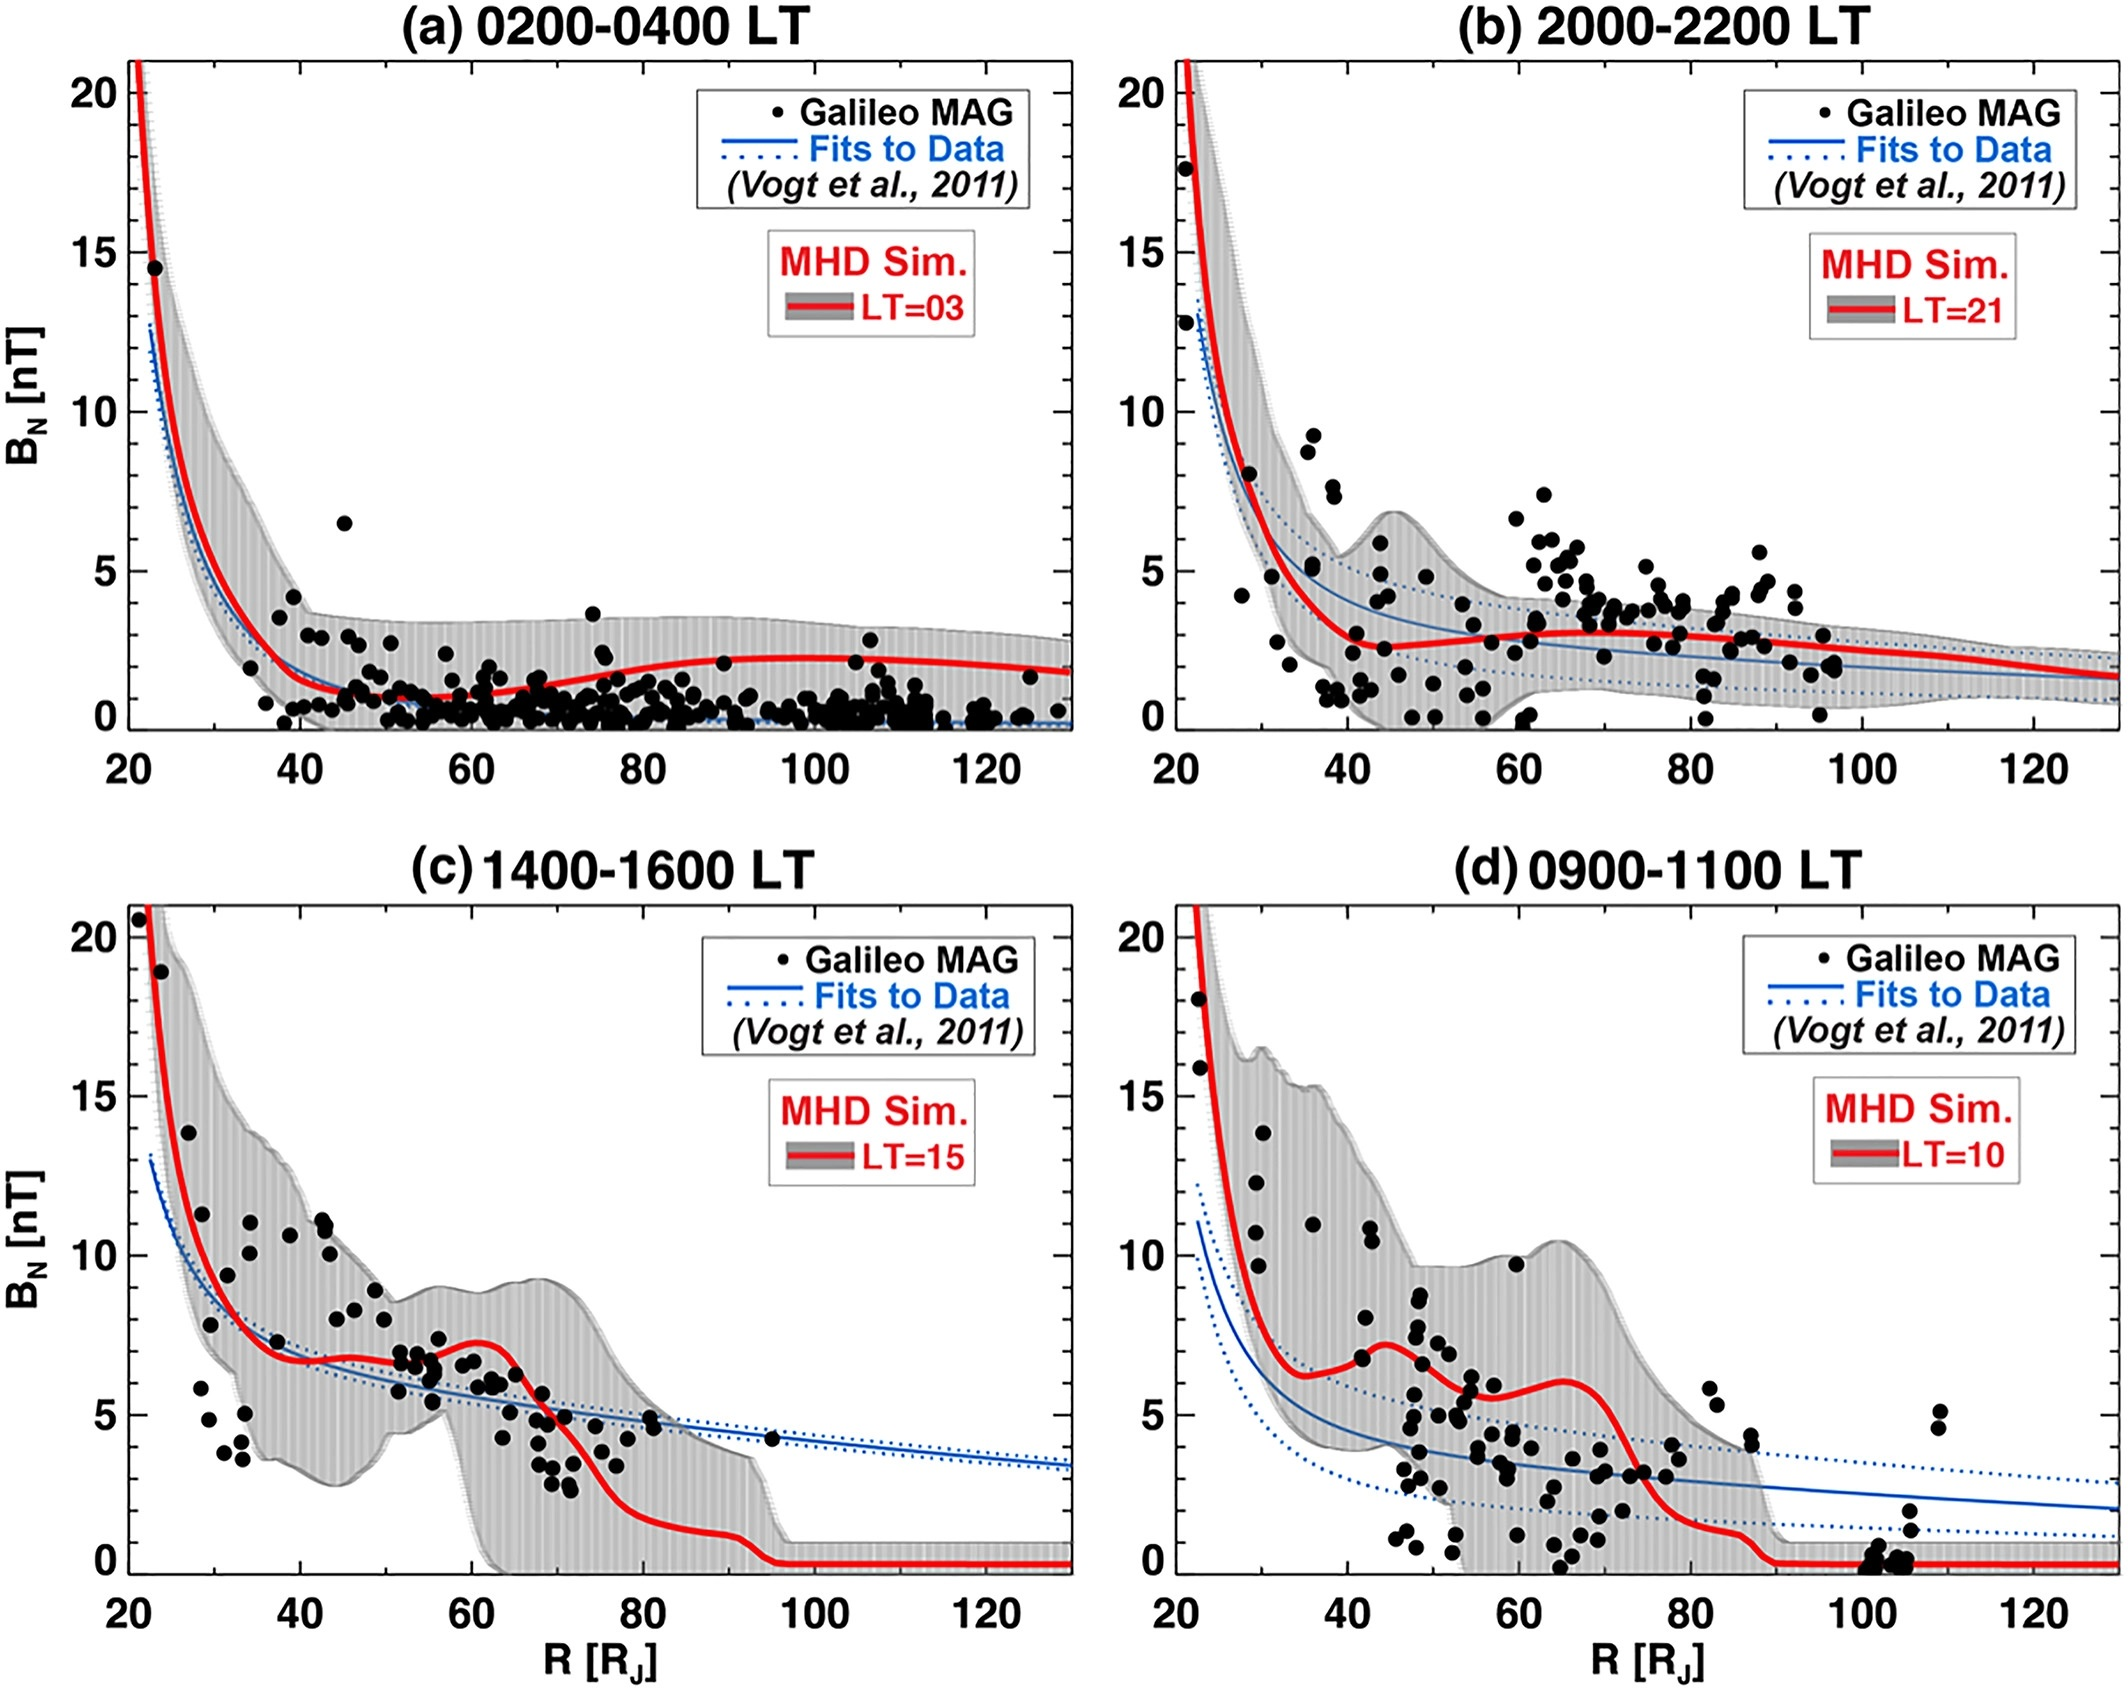
\includegraphics[width=\textwidth]{images2/comparison-magneticfield.jpg}
    \caption{In each panel, the black dots show observations of the magnetic field component ($B_N$) normal to the current sheet, and the blue solid and dashed lines show fits to the data (adapted from \protect\citeNP{Vogt2011a}). The red line in each panel represents the average radial profile of $B_N$ output from our magnetohydrodynamic (MHD) simulation in the same local time sector as the data were collected, and the grey bars in the background show the range of values seen at different simulation times in our global model. (Figures adapted from \protect\citeNP{Vogt2011a})}
    \label{fig:comparison-magneticfield}
\end{figure}

In addition to the plasma parameters, we also compare our simulated magnetic field with observations. As an example, Figure \ref{fig:comparison-magneticfield} presents a comparison of the magnetic field component normal to the current sheet ($B_N$ ) to the data collected by previous missions, including Pioneer, Voyager, Ulysses, and Galileo \cite{Vogt2011a}. This data set was the basis of the magnetic field model (fits to the data shown as blue curves in the figure) developed by \cite{Vogt2011a} that allows to map regions in the magnetosphere to the ionosphere. The observational data were shown in different local time bins; thus, we extracted our model results from the same local time sectors correspondingly. Since there are time‐varying structures formed in our simulation even under steady upstream conditions, we show both the time‐averaged radial profiles and the range of $B_N$ seen in our simulation. Overall, our model result follows the trends of the $B_N$ variation quite well in all local time sectors compared. Comparing the ranges of our modeled $B_N$ with the data also shows that much of the scattering in the data could potentially be attributed to temporal variations of the magnetosphere and/or changes due to external conditions. Moreover, our model captures very well the observed local time asymmetry in $B_N$ (weak on the dawnside and strong on the duskside), indicative of the different thicknesses of the current sheet between dawn and dusk that have been identified previously \cite{Khurana2005,Kivelson2002a}.

\section{Limitations of the model}
We note that the global simulations presented here are based on an ideal MHD model, which does not capture non-ideal MHD processes, such as energy‐dependent particle drifts, temperature anisotropy, and kinetic physics involved in magnetic reconnection. While no simulation can fully model the complexity of a planetary magnetosphere, extensive prior work has demonstrated that MHD models generally can provide a reasonably good representation of the global structure of a planetary magnetosphere whose size is much larger than the characteristic ion spatial scales, which is the case for Jupiter. This is true, because while magnetic reconnection occurs due to numerical resistivity in the model, it generally occurs at the right location where the current sheets carry strong currents (numerically represented by a jump in the magnetic field) and approximately with the correct reconnection rate that is some fraction ($\sim$0.1) of the Alfven speed (the numerical diffusion term is proportional with the local maximum wave speed); therefore, the global solution is expected to be approximately right. The main goal of this study is to investigate the large‐scale response of Jupiter's coupled magnetosphere‐ionosphere system to solar wind drivers, for which an MHD model is a suitable tool.

\section{Summary}
We have developed a new MHD model for Jupiter's magnetosphere using the BATSRUS MHD code. To validate the model, we compared the modeled density, velocity, thermal pressure, magnetic field, and plasma $\beta$ extracted from multiple time steps and from simulation runs with different external conditions with available in situ observations and found generally good agreements. In particular, while our model under-predicts the plasma density (and pressure) in the inner magnetosphere ($<10 R_J$) due to potential reasons of grid resolution and/or the assumption of isotropic pressure in ideal MHD, our model results match very well the statistical results from observations outside of 10 $R_J$ in terms of plasma density, azimuthal velocity, and the magnetic field. Further, our model also captures the dawn‐dusk asymmetries in the thickness of the current sheet \cite{Khurana2005,Vogt2011a} as observed by the Galileo spacecraft, that is, thicker current sheet on the dusk-side compared to dawn. The locations of the magnetopause and bow shock in our model are also generally consistent with the predictions by the empirical models of \cite{Joy2002a}, although our simulated magnetopause is slightly smaller in size due to the lack of energetic particles in the MHD model. 